\chapter{Технологический раздел}
\label{cha:impl}

В данном разделе описывается стек технологий, графический конвейер, структура программы и ее интерфейс.

\section{Выбор и обоснование языка программирования и среды разработки}

Язык программирования: C++, glsl

Библиотеки: vulkan, imgui (gui библиотека), glm (математическая библиотека), libxcb (linux)

Редактор: VSCode

Система автоматизации сборки: CMake
\\

Приоритет для рендеринга в реальном времени - скорость и производительность.
Поэтому я использую C ++, поддерживаю объектно-ориентированное программирование и гарантирую высокую скорость, хорошее взаимодействие с графическим API Vulkan.

% C++ use for interacting with user, glsl get compile to 


\begin{itemize}
    \item Vukan: графический и вычислительный API нового поколения,
    обеспечивающий высокоэффективный кроссплатформенный доступ к
    современным графическим процессорам, используемым в разных устройствах.
    Целью Vulkan было превзойти другие API, включая его предшественника OpenGL,
    в части снижения накладных расходов, повышения степени прямого контроля над GPU и уменьшения нагрузки на CPU.

    \item ImGui: Графический пользовательский интерфейс немедленного режима,
    представляет собой шаблон проектирования графического пользовательского интерфейса,
    который использует графическую библиотеку немедленного режима
    для создания графического интерфейса.

    \item libvkbase: Поскольку время ограничено, а Vulkan - это графический api
    низкого уровня, я буду использовать репозиторий на github, используя некоторые
    очень хорошо абстрактные файлы (рекомендованные создателями vulkan)
    (только те, которые мне нужны). Оттуда я создаю статическую библиотеку libvkbase и использую ее.
    
    \item Программное обеспечение было разработано для Linux, но его можно
    продолжать развиваться как для MacOS, так и для Windows.
\end{itemize}

\section{Описание программы}

Программа объектно-ориентированная, но не полностью.
Для простоты игнорируются некоторые принципы объектно-ориентированного программирования.
Одним из доказательств полезности объектно-ориентированного программирования является то,
что программа легко расширяется и поддерживает форматы файлов.


% \subsection*{Графический конвейер}
\subsection*{Рабочий конвейер программы}

\begin{figure}[H]
    \centering
    \includegraphics[width=0.8\textwidth]{img/cg.png}
    \caption{Рабочий конвейер программы}
    \label{fig:3.1}
\end{figure}


\subsection*{Формат входных данных}

В качестве формат входных данных, используется формат .obj.
Это широко используемый формат с открытым исходным кодом.
Формат файла obj имеет много свойств, но нас интересуют только два свойства:

\begin{verbatim}
    # Список вершин, с координатами
    v 0.000 0.500 1.000
    v ...

    # Определения поверхности
    f 1 2 3
    f 3/1 4/2 5/3
    f 6/4/1 3/5/3 7/6/5
    f 6//1 3//3 7//5
    f ...
\end{verbatim}

При загрузке использование класса Parser считывает в модель файл в формате obj.
Модель преобразуется в массив треугольников и сохранит его в сцене.


\section{Описание структуры программы}

\begin{itemize}
    \setlength{\itemsep}{0em}
    \item data/: Содержит скомпилированные шейдеры, шрифты и файл модели (алмаза), требуется при запуске программы.
    \item lib/: Содержит необходимые библиотеки. (imgui, libvulkan, libxcb)
    \item shaders/: Содержит исходный код вычислительных шейдеров.
    \begin{itemize}
        \item ray/
        \begin{itemize}
            \item entity.glsl : Описывает структуры данных, хранящиеся в графическом процессоре.
            \item intersect.glsl : Обработка пересечений
            \item light.glsl : Обработка окраски
            \item rt.comp : Точка входа в вычисление шейдера
            \item ...
        \end{itemize}
        \item ui/: Шейдеры для пользовательского интерфейса
    \end{itemize}
    \item src/: Содержит исходный код C++
    \begin{itemize}
        \item Model/
        \begin{itemize}
            \item camera.h: Класс Camera
            \item entity.h: Описание геометрических объектов
            \item material.h: Описание материалов и хранение материалов
            \item model.h: Класс Model
            \item parser.h, parser.cpp, parser\_handler.h: Парсер файла модели
            \item scene.h, scene.cpp: Управлять всеми объектами в сцене.
        \end{itemize}
        \item vulkanbase.h, vulkanbase.cpp: абстрактный класс приложения vulkan
        \item app.h
        \item app\_ui.cpp: Пользовательский интерфейс
        \item app\_vulkan.cpp: Процедуры связанных с vulkan
        \item main.cpp: настроить камеру и создать сцену
        \item keycodes.h
        \item entrypoint.h
    \end{itemize}
    \item vkbase/: Файлы, используемые для сборки libvkbase. Отредактировано и усечено для уменьшения размера файла.
    \item CMakeLists.txt
    \item run.sh: Скрипт помогает быстро собрать, запустить и протестировать
\end{itemize}

Программный продукт состоит из двоичного файла \textbf{app} и папки \textbf{data/}, содержащей скомпилированные шейдеры, шрифты и файл модели (алмаза).


\section{Интерфейс программы}

Я использую Dear Imgui - библиотеку графического пользовательского интерфейса для C ++,
она выводит оптимизированные буферы вершин (в данном случае визуализируется в графическом интерфейсе приложения vulkan).
Ниже приводится описание интерфейса и его снимки (рисунок \ref{fig:3.1} и \ref{fig:3.2}).

\begin{itemize}
    \item Отладочная информация
    \begin{itemize}
        \item Видеокарта
        \item Кадров в секунду (fps)
    \end{itemize}
    \item Менеджер сцены
    \begin{itemize}
        \item Точечный источник света: можно изменить цвет света и интенсивность света
        \item Интенсивность окружающего света
        \item Камера: может менять положение
        \item Максимальное количество раз отскока луча
        \item Список объектов в сцене (сферы, плоскости, кубы, алмаз)
    \end{itemize}
    \item Менеджер объектов
    \begin{itemize}
        \item Добавить объект: сфера, куб
        \item Изменить объект: в зависимости от выбранного объекта могут быть
    изменены соответствующие параметры
        \item Изменить материал: свет, $k_a, k_d, k_s, shininess, k_{reflect}, ior$
        \item Можно выбрать материал из списка определенных материалов.
    \end{itemize}
    \item Угол камеры можно легко изменить с помощью мыши, а движение источника света останавливается нажатием клавиши P.
    \item Интерфейс можно свернуть, чтобы не занимать область отображения (рис. \ref{fig:3.2})
\end{itemize}


\begin{figure}[h]
    \centering
    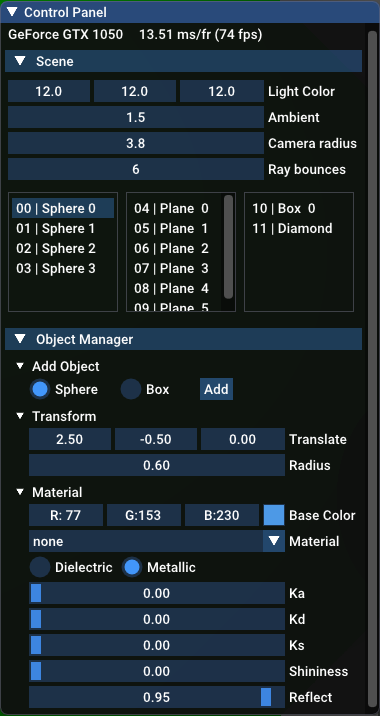
\includegraphics[width=0.5\textwidth]{img/screenshot/ui1.png}
    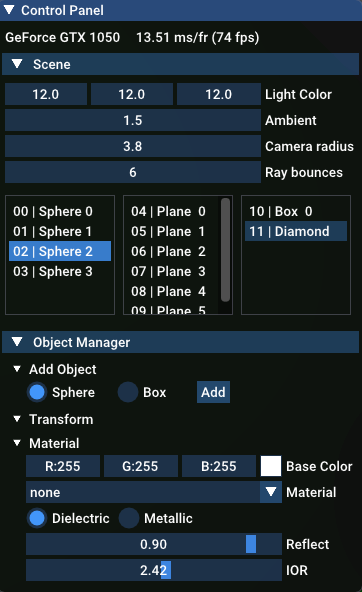
\includegraphics[width=0.46\textwidth]{img/screenshot/ui2.png}
    \caption{Интерфейс программы меняется в зависимости от выбранного объекта}
    \label{fig:3.1}
\end{figure}

\begin{figure}[h]
    \centering
    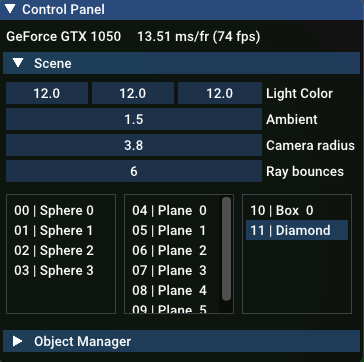
\includegraphics[width=0.5\textwidth]{img/screenshot/ui3.png}
    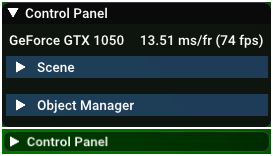
\includegraphics[width=0.4\textwidth]{img/screenshot/ui4.png}
    \caption{Интерфейс можно свернуть, чтобы не занимать область отображения}
    \label{fig:3.2}
\end{figure}
